% -------------------------------------------------------------------------
%  MusicFormats Library
%  Copyright (C) Jacques Menu 2016-2023

%  This Source Code Form is subject to the terms of the Mozilla Public
%  License, v. 2.0. If a copy of the MPL was not distributed with this
%  file, you can obtain one at http://mozilla.org/MPL/2.0/.

%  https://github.com/jacques-menu/musicformats
% -------------------------------------------------------------------------

% !TEX root = MusicFormatsUserGuide.tex

% -------------------------------------------------------------------------
\chapter{MusicFormats installation modes}
% -------------------------------------------------------------------------

There is no GUI installer available yet, so users have to install the library at a lower level, sorry for that\dots.

How to install \mf\ depends on the \OS. \Linux\ users often build the software they use themselves, while those of \Windows\ and \MacOS\ are accustomed to install in much simpler ways.

Depending on the needs, users may wish to install the \MainIt{whole} \mf\ with documentation, source code and examples, or to use a {\it \readyToUseVersion}, that contains only the binary \MainIt{libraries}, the \CLI\ executables and the documentation \pdf\ files.

The following chapters show the details.


% -------------------------------------------------------------------------
\chapter{Using a ready-to-use version}
% -------------------------------------------------------------------------

\mf\ comes with  \readyToUseVersion s for \MacOS, \Ubuntu\ and \Windows\ in the form of \zip\ files., including the user documentation PDF file. \fileName{MusicFormatsVersionNumber.txt} contains the library's version number, while \fileName{MusicFormatsVersionDate.txt} contains its release date.


There are eady-to-use versions of \mf\ for the three main operating systems,
i.e. MacOS™, Linux in its Ubuntu declination and Windows™.
They are in ZIP format and can be downloaded from the repository main page at
\url{https://github.com/jacques-menu/musicformats}.
Click on the 'n tags' link at the top of the page to access the various versions.

One can also go directly to:
\url{https://github.com/jacques-menu/musicformats/tags}.
Then click on the link to the desired version such as v0.9.65, to access its contents.

Each \code{.zip} archive contains:
\begin{itemize}
\item  text files containing the version number and release date;
\item  the executable tools ans services in the bin subdirectory;
\item  binary versions of the library in the lib subdirectory;
\item  a PDF introduction to MusicXML;
\item  a PDF MusicFormats user guide.
\end{itemize}

These ready-to-use versions can be accessed directly with URLs such as:
\url{https://github.com/jacques-menu/musicformats/releases/tag/v0.9.65}.
Replace v0.9.65 by the version number for the desired operations system.

Their contents is, for example, the following. The dots in the version number are replaced by underscores due to a GitHub feature:\\
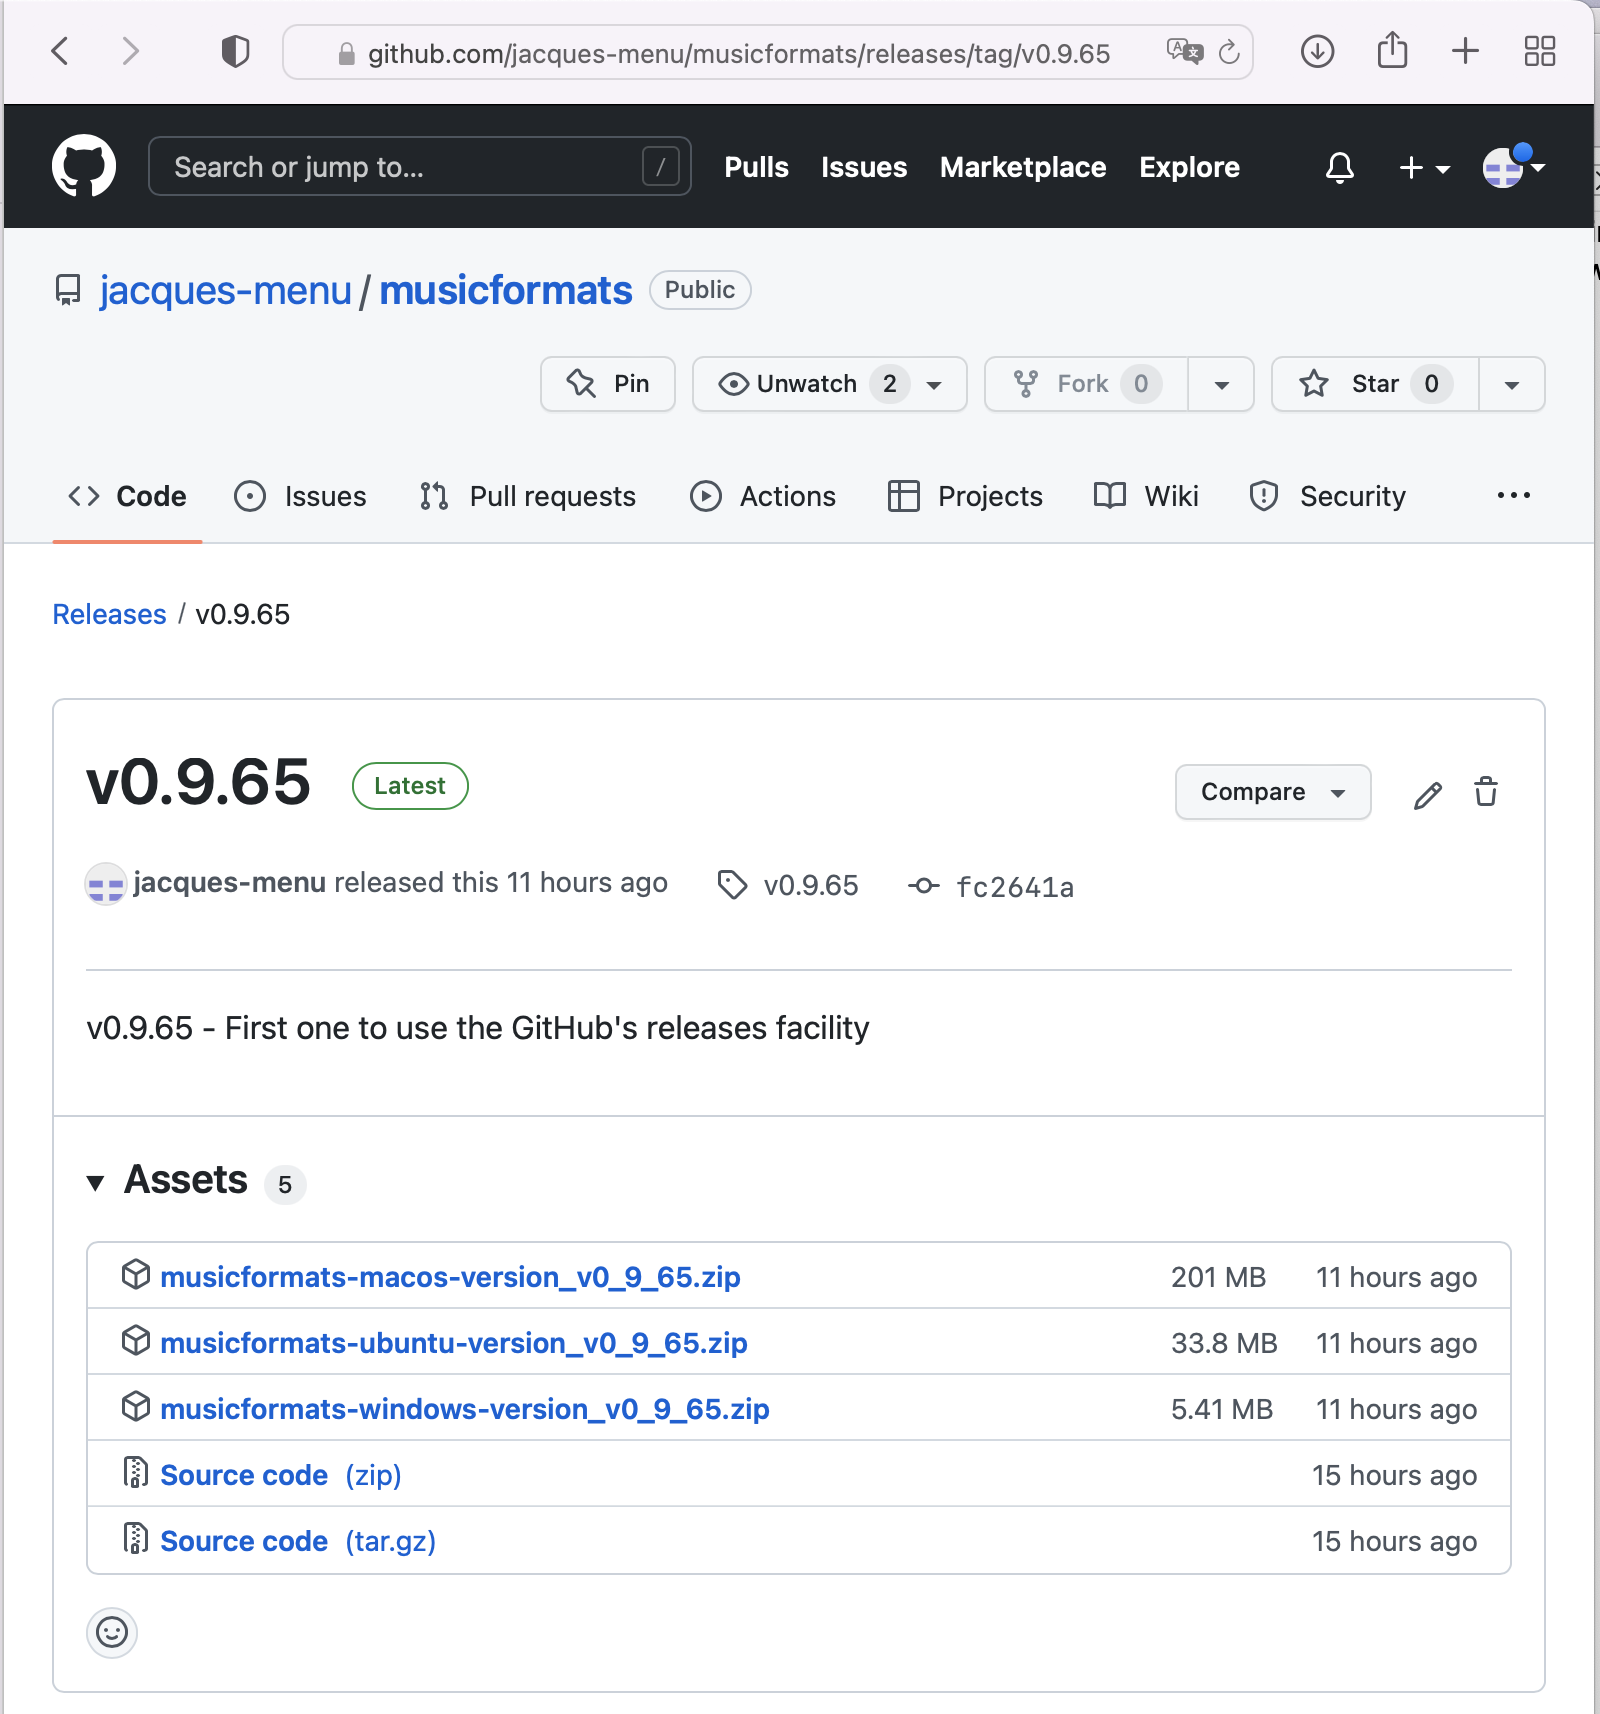
\includegraphics[scale=0.5]{../graphics/ReadyToUseVersionContents.png}

Once uncompressed on the user's machine, the contents looks like:\\
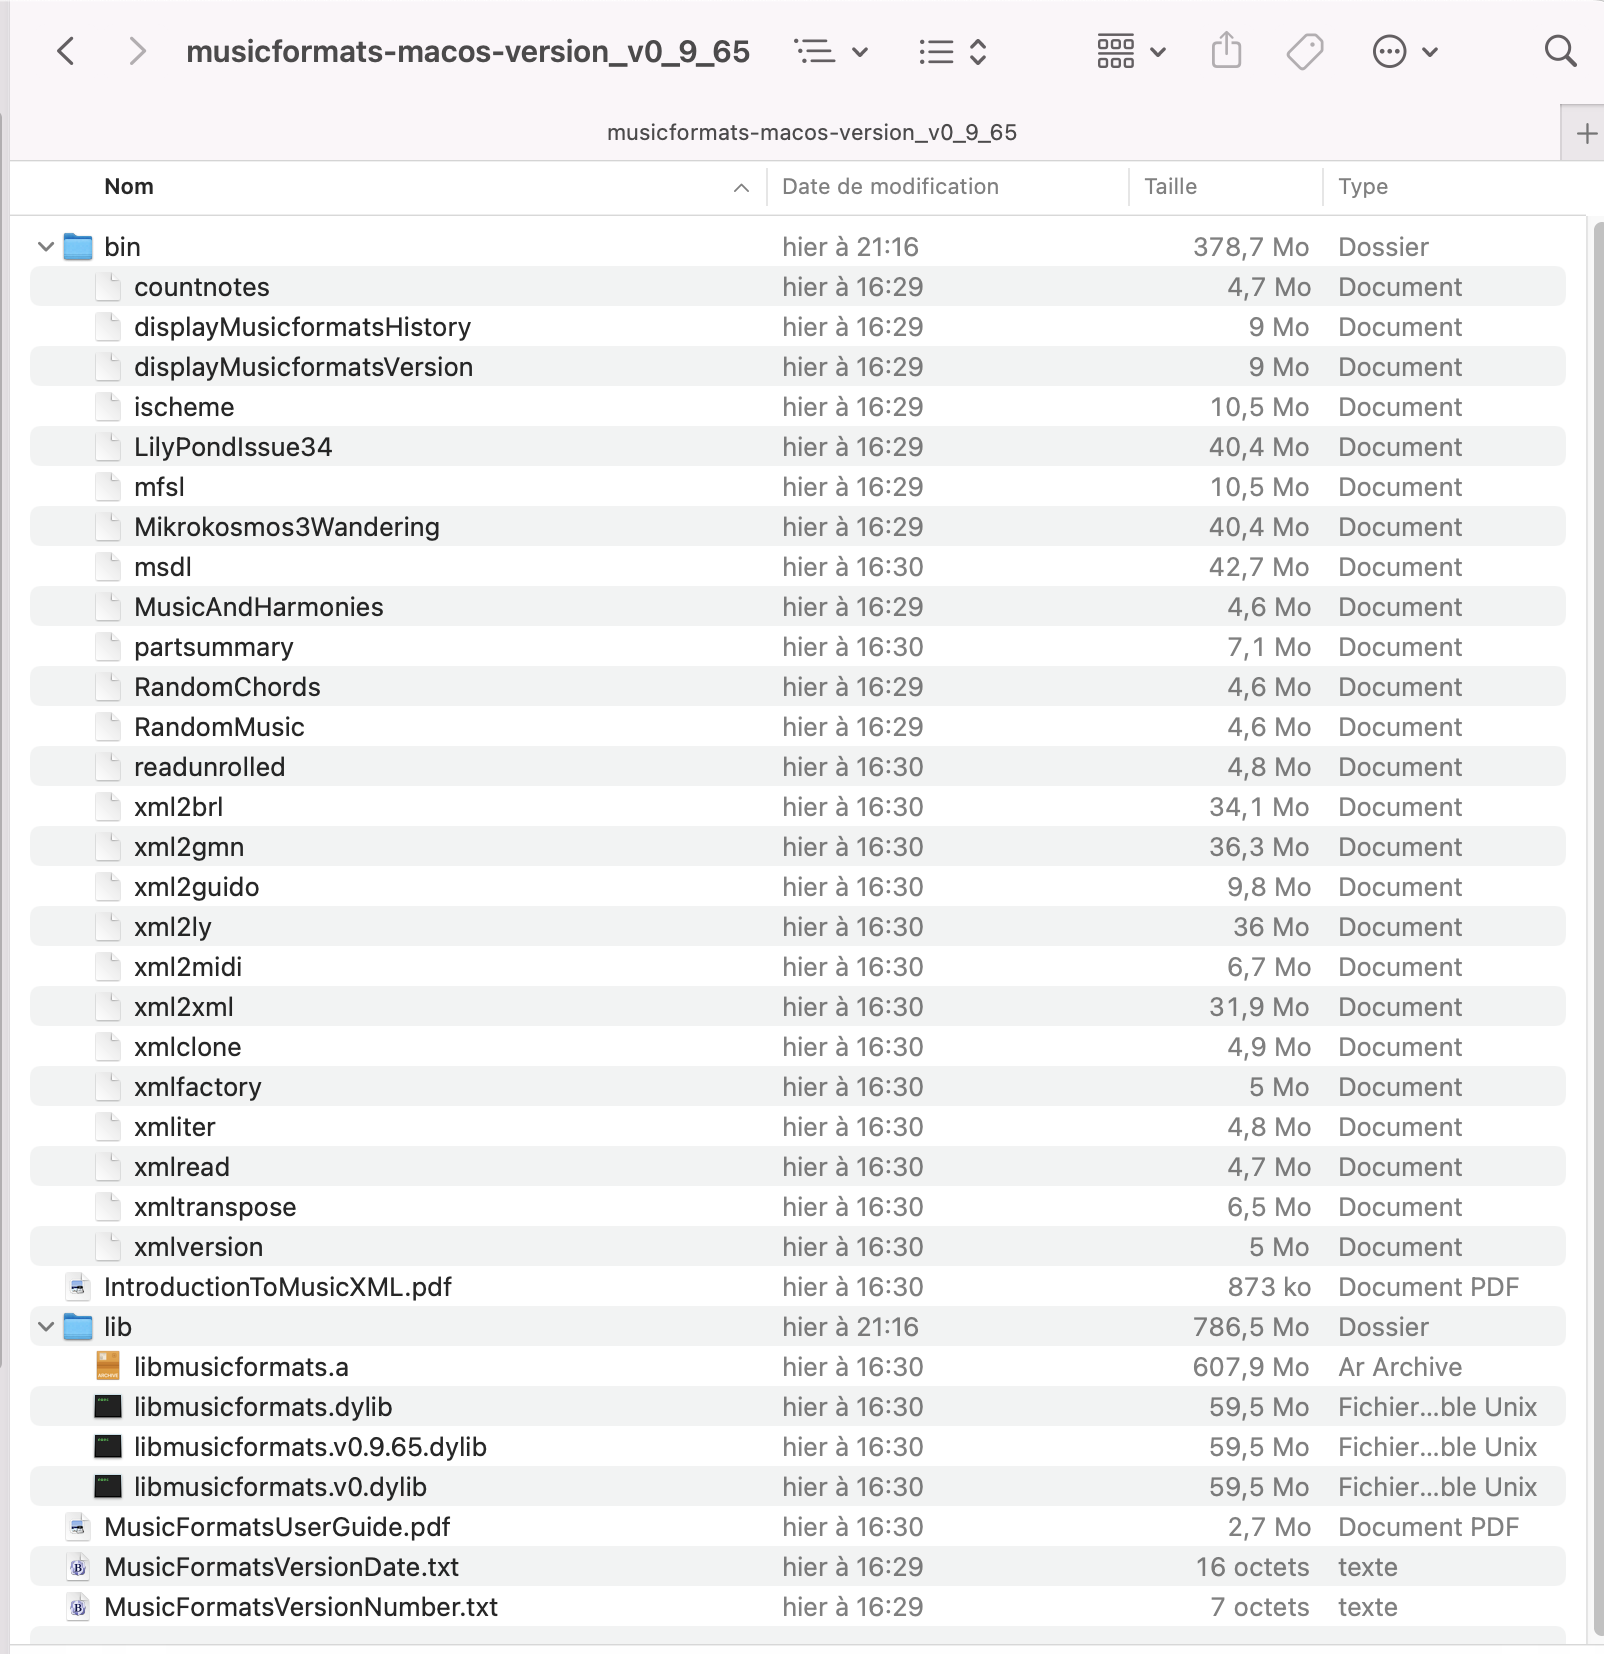
\includegraphics[scale=0.5]{../graphics/ReadyToUseVersionContentsExample.png}


% -------------------------------------------------------------------------
\section{Using the MacOS\texttrademark\ ready-to-use version}
% -------------------------------------------------------------------------

\MacOS\ software is usually distributed as \Main{DMG} files. Due to file size limitations on \github, the \MacOS\ \readyToUseVersion has to be compacted. This is done with \zip, and placing that in a DMG archive would not add any value. Only the \zip\ archive is thus provided.

%%%JMI\mf\ is  installable directly from the repository, since this is the environment is is developed on. Just clone the \repo\ and you will find the executables in \build{bin} and the libraries in \build{lib}.

After downloading and uncompressing \fileName{musicformats-macos-version_v0_9_65.zip}, we get:
\begin{lstlisting}[language=Terminal]
jacquesmenu@macmini:~/musicformats-git-dev/readytouse/musicformats-macos-version_v0_9_65 > ls -salR
total 7072
   0 drwxr-xr-x   9 jacquesmenu  staff      288 Aug 23 21:39 .
   0 drwxr-xr-x   6 jacquesmenu  staff      192 Aug 24 09:03 ..
  16 -rw-r--r--@  1 jacquesmenu  staff     6148 Aug 24 09:04 .DS_Store
1712 -rw-r--r--@  1 jacquesmenu  staff   872863 Aug 23 16:30 IntroductionToMusicXML.pdf
5328 -rw-r--r--@  1 jacquesmenu  staff  2726266 Aug 23 16:30 MusicFormatsUserGuide.pdf
   8 -rw-r--r--@  1 jacquesmenu  staff       16 Aug 23 16:29 MusicFormatsVersionDate.txt
   8 -rw-r--r--@  1 jacquesmenu  staff        7 Aug 23 16:29 MusicFormatsVersionNumber.txt
   0 drwxr-xr-x@ 27 jacquesmenu  staff      864 Aug 23 21:16 bin
   0 drwxr-xr-x@  6 jacquesmenu  staff      192 Aug 23 21:16 lib

./bin:
total 739832
    0 drwxr-xr-x@ 27 jacquesmenu  staff       864 Aug 23 21:16 .
    0 drwxr-xr-x   9 jacquesmenu  staff       288 Aug 23 21:39 ..
78904 -rw-r--r--@  1 jacquesmenu  staff  40397088 Aug 23 16:29 LilyPondIssue34
78912 -rw-r--r--@  1 jacquesmenu  staff  40400272 Aug 23 16:29 Mikrokosmos3Wandering
 9024 -rw-r--r--@  1 jacquesmenu  staff   4616384 Aug 23 16:29 MusicAndHarmonies
 9024 -rw-r--r--@  1 jacquesmenu  staff   4616368 Aug 23 16:29 RandomChords
 9024 -rw-r--r--@  1 jacquesmenu  staff   4616368 Aug 23 16:29 RandomMusic
 9216 -rw-r--r--@  1 jacquesmenu  staff   4717184 Aug 23 16:29 countnotes
17616 -rw-r--r--@  1 jacquesmenu  staff   9017664 Aug 23 16:29 displayMusicformatsHistory
17616 -rw-r--r--@  1 jacquesmenu  staff   9017664 Aug 23 16:29 displayMusicformatsVersion
20440 -rw-r--r--@  1 jacquesmenu  staff  10464016 Aug 23 16:29 ischeme
20424 -rw-r--r--@  1 jacquesmenu  staff  10455664 Aug 23 16:29 mfsl
83344 -rw-r--r--@  1 jacquesmenu  staff  42669776 Aug 23 16:30 msdl
13960 -rw-r--r--@  1 jacquesmenu  staff   7143520 Aug 23 16:30 partsummary
 9416 -rw-r--r--@  1 jacquesmenu  staff   4817280 Aug 23 16:30 readunrolled
66568 -rw-r--r--@  1 jacquesmenu  staff  34080976 Aug 23 16:30 xml2brl
70848 -rw-r--r--@  1 jacquesmenu  staff  36271984 Aug 23 16:30 xml2gmn
19224 -rw-r--r--@  1 jacquesmenu  staff   9841744 Aug 23 16:30 xml2guido
70320 -rw-r--r--@  1 jacquesmenu  staff  36002128 Aug 23 16:30 xml2ly
13024 -rw-r--r--@  1 jacquesmenu  staff   6666832 Aug 23 16:30 xml2midi
62304 -rw-r--r--@  1 jacquesmenu  staff  31898736 Aug 23 16:30 xml2xml
 9664 -rw-r--r--@  1 jacquesmenu  staff   4944768 Aug 23 16:30 xmlclone
 9848 -rw-r--r--@  1 jacquesmenu  staff   5039760 Aug 23 16:30 xmlfactory
 9392 -rw-r--r--@  1 jacquesmenu  staff   4808640 Aug 23 16:30 xmliter
 9240 -rw-r--r--@  1 jacquesmenu  staff   4728176 Aug 23 16:30 xmlread
12632 -rw-r--r--@  1 jacquesmenu  staff   6463856 Aug 23 16:30 xmltranspose
 9848 -rw-r--r--@  1 jacquesmenu  staff   5039216 Aug 23 16:30 xmlversion

./lib:
total 1536144
      0 drwxr-xr-x@ 6 jacquesmenu  staff        192 Aug 23 21:16 .
      0 drwxr-xr-x  9 jacquesmenu  staff        288 Aug 23 21:39 ..
1187400 -rw-r--r--@ 1 jacquesmenu  staff  607947008 Aug 23 16:30 libmusicformats.a
 116248 -rw-r--r--@ 1 jacquesmenu  staff   59514976 Aug 23 16:30 libmusicformats.dylib
 116248 -rw-r--r--@ 1 jacquesmenu  staff   59514976 Aug 23 16:30 libmusicformats.v0.9.65.dylib
 116248 -rw-r--r--@ 1 jacquesmenu  staff   59514976 Aug 23 16:30 libmusicformats.v0.dylib
\end{lstlisting}

\MacOS\ executables are self-sufficient and can be placed anywhere on a disk except the trash. Usually, they are placed in the \code{/Applications} directory.


% -------------------------------------------------------------------------
\subsection{Security issue in recent MacOS\texttrademark\ versions}
% -------------------------------------------------------------------------

\MacOS\ gets more and more stringent over time regarding security. The \OS\ part in charge of this is named \Gatekeeper.

When installing \mf\ from the \repo\ on versions up to 10 (\Main{High Sierra}), the executables in \code{bin} are usable alright.

From version 11 (\Main{Catalina}) on, though, the executables you get are not executable actually, because their developer is unknown to the \OS, and actions have to be taken for them to be usable.

The screenshot below has been made with \MacOS\ \Main{Monterey} 12.0.1 with english as the user interface language. The texts vary of course depending on the language used.

When launching one of these executables for the first time, such as:
\begin{lstlisting}[language=Terminal]
jacquesmenu@macmini: ~/Downloads/MusicFormatsForMacOS/bin > ./xml2ly
\end{lstlisting}
we get a alert telling that it cannot be opened, because the developper is not known to the \OS:\\
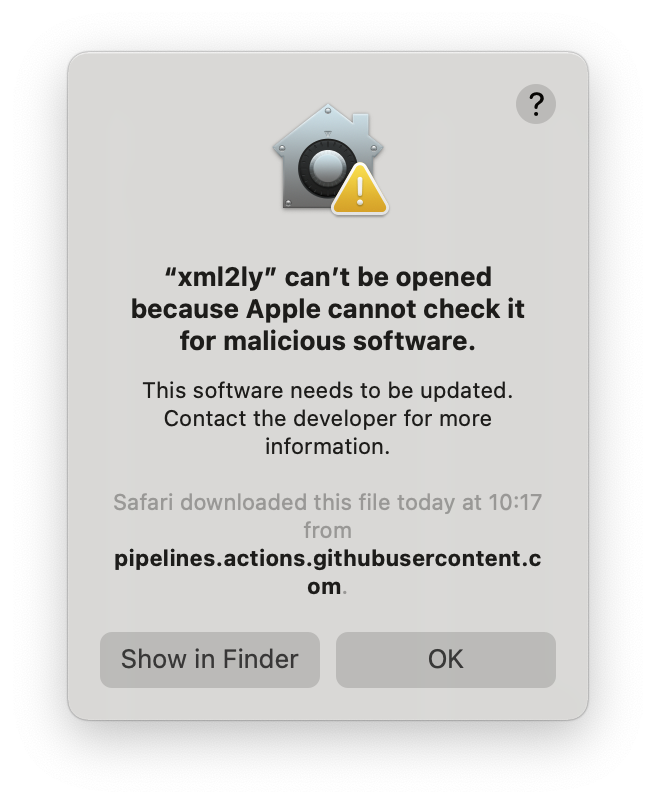
\includegraphics[scale=0.35]{../graphics/MacOSMaliciousSoftwareAlert.png}

Clicking in either buttons in this dialog kill the process:
\begin{lstlisting}[language=Terminal]
Killed: 9
\end{lstlisting}

The trouble is that these executables are in {\it \quarantine} by default. To make them usable, they have to quit quarantine, which is done by removing one of their attributes:
\begin{lstlisting}[language=Terminal]
jacquesmenu@macmini: ~/Downloads/MusicFormatsForMacOS/bin > xattr -d com.apple.quarantine *
\end{lstlisting}
%codesign --sign - --force --deep %%%JMI not necessary

From then on, the \mf\ executables can be used seamlessly on the given machine.

Having to perform the preceding task for each executable is the price to pay for security. And it has to be perfomed again when installing new versions\dots


The above can be done in the \GUI\ file by file too. Right after you got the message above:
\begin{itemize}
\item  open \MainIt{System Preferences}, choose the \MainIt{Security \& Privacy} tab, and there click on the \MainIt{General button};

\item click on the lock at the bottom left of the dialog to make changes:\\
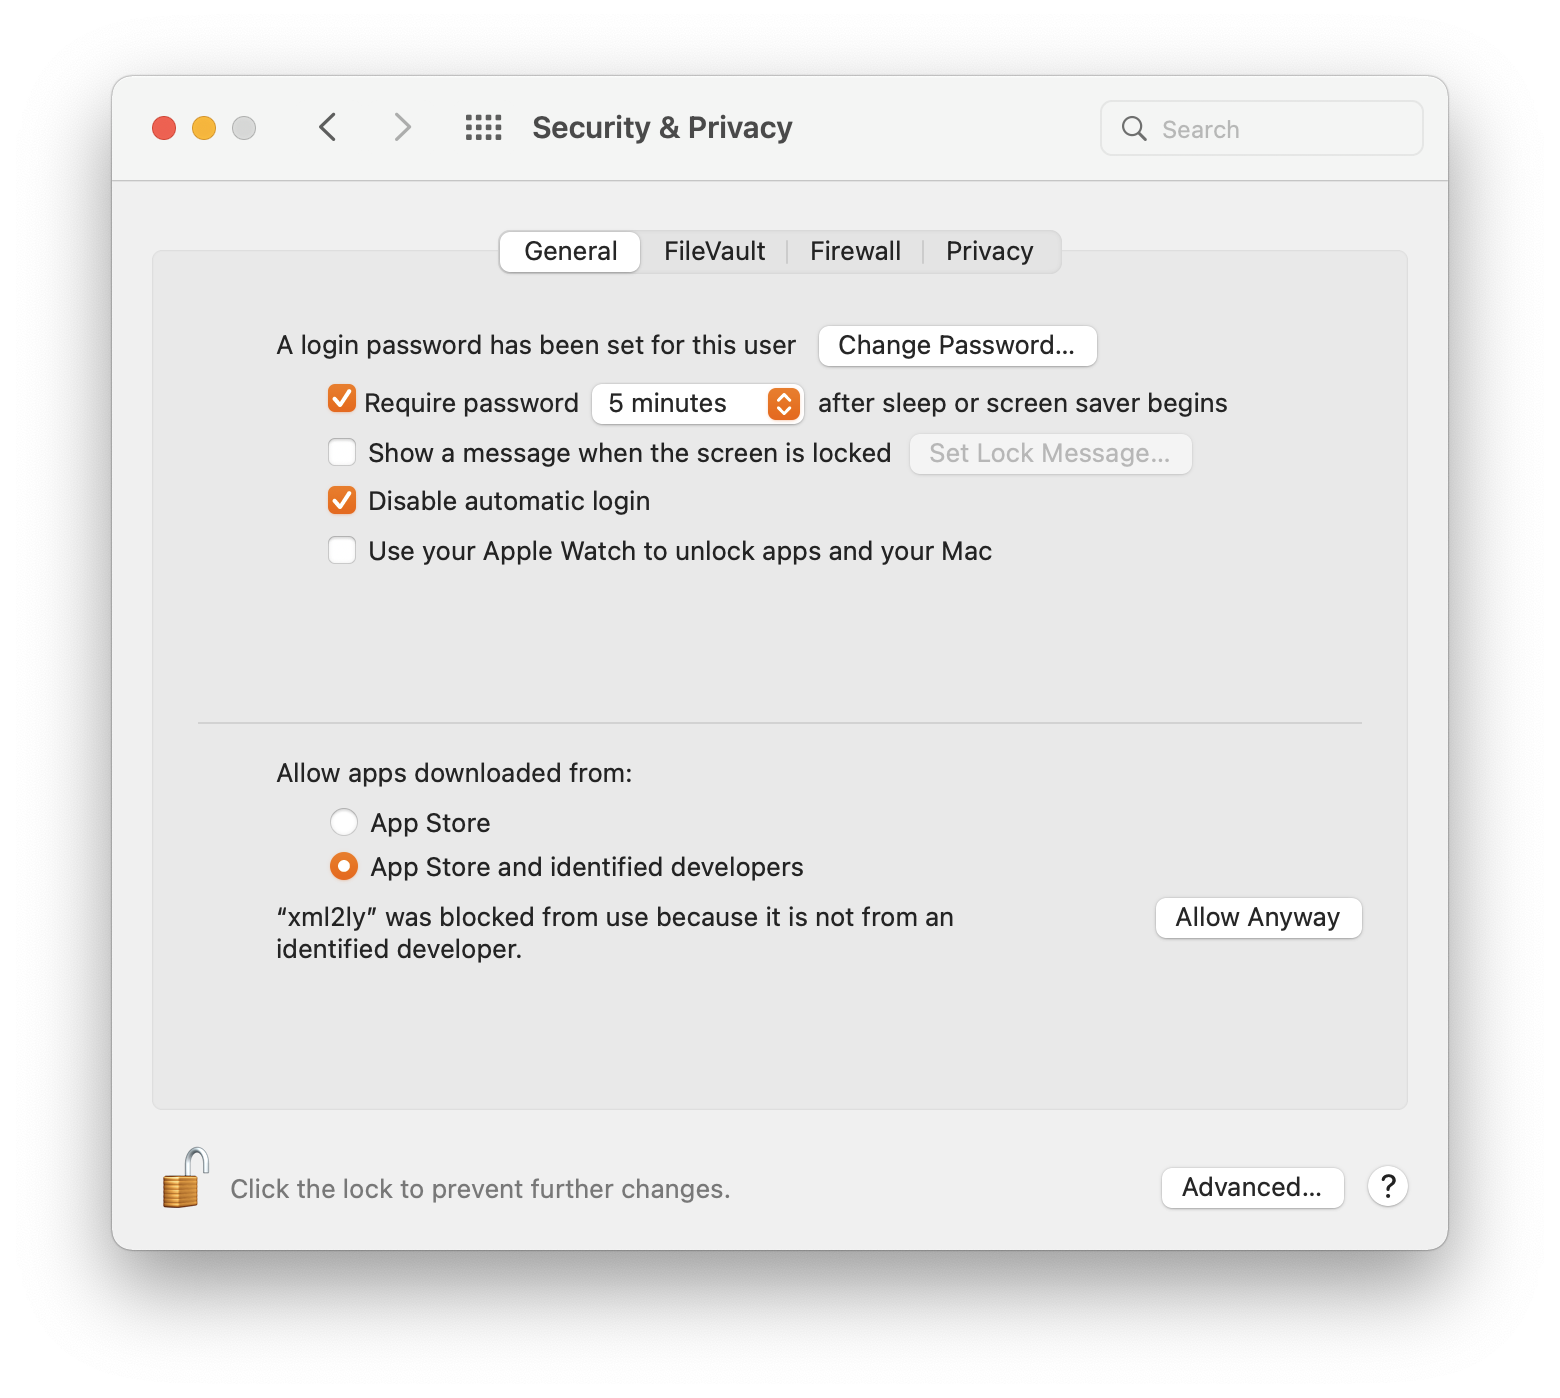
\includegraphics[scale=0.35]{../graphics/MacOSAllowAnyway.png}

\item click on the \MainIt{Allow Anyway} button.
%%%JMI sudo spctl --master-disable to create a Anywhere radio button
%jacquesmenu@macmini > spctl --status
%assessments enabled

\end{itemize}

Re-execute the executable from the command line. This pops-up a dialog to confirm you actually want to use this software:\\
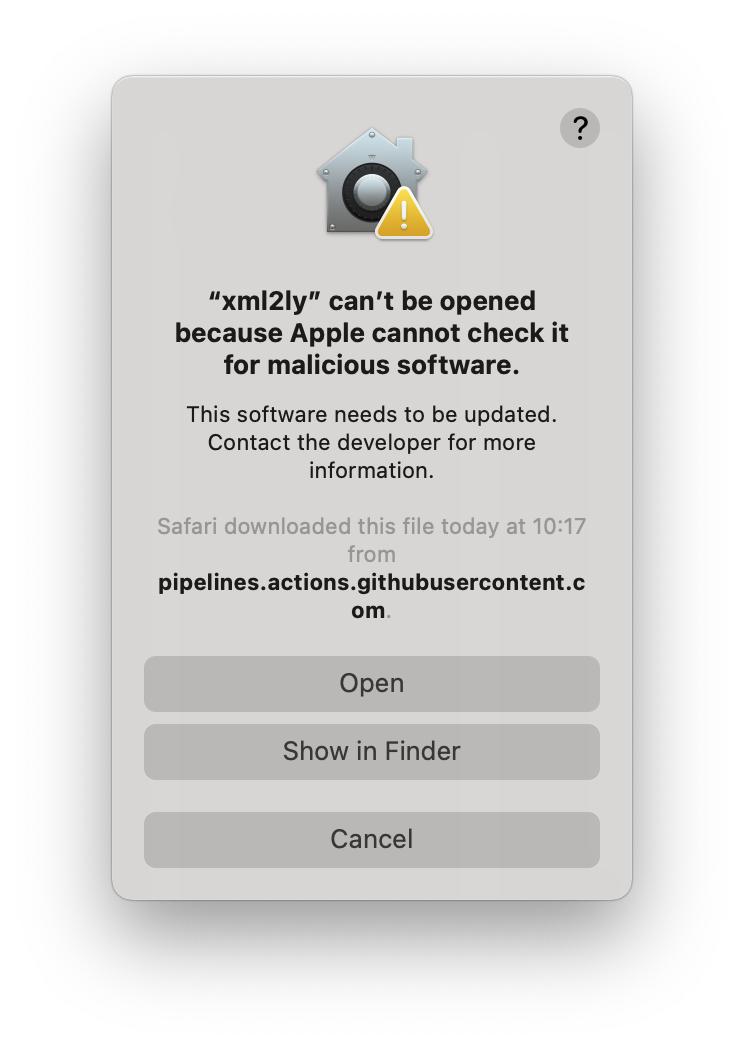
\includegraphics[scale=0.35]{../graphics/MacOSConfirmOpening.png}

Click on the \MainIt{Open} button to register the executable in \Gatekeeper\ and go ahead.


% -------------------------------------------------------------------------
\section{Using the Ubuntu ready-to-use version}
% -------------------------------------------------------------------------

After downloading and uncompressing \fileName{musicformats-ubuntu-version_v0_9_65.zip}, we get:
\begin{lstlisting}[language=Terminal]
jacquesmenu@macmini:~/musicformats-git-dev/readytouse/musicformats-ubuntu-version_v0_9_65 > ls -salR
total 7072
   0 drwxr-xr-x   9 jacquesmenu  staff      288 Aug 23 21:39 .
   0 drwxr-xr-x   6 jacquesmenu  staff      192 Aug 24 09:03 ..
  16 -rw-r--r--@  1 jacquesmenu  staff     6148 Aug 24 09:03 .DS_Store
1712 -rw-r--r--@  1 jacquesmenu  staff   872863 Aug 23 16:45 IntroductionToMusicXML.pdf
5328 -rw-r--r--@  1 jacquesmenu  staff  2726266 Aug 23 16:45 MusicFormatsUserGuide.pdf
   8 -rw-r--r--@  1 jacquesmenu  staff       16 Aug 23 16:45 MusicFormatsVersionDate.txt
   8 -rw-r--r--@  1 jacquesmenu  staff        7 Aug 23 16:45 MusicFormatsVersionNumber.txt
   0 drwxr-xr-x@ 27 jacquesmenu  staff      864 Aug 23 21:15 bin
   0 drwxr-xr-x@  6 jacquesmenu  staff      192 Aug 23 21:15 lib

./bin:
total 2344
  0 drwxr-xr-x@ 27 jacquesmenu  staff     864 Aug 23 21:15 .
  0 drwxr-xr-x   9 jacquesmenu  staff     288 Aug 23 21:39 ..
 96 -rw-r--r--@  1 jacquesmenu  staff   48944 Aug 23 16:45 LilyPondIssue34
 96 -rw-r--r--@  1 jacquesmenu  staff   48984 Aug 23 16:45 Mikrokosmos3Wandering
 96 -rw-r--r--@  1 jacquesmenu  staff   47280 Aug 23 16:45 MusicAndHarmonies
 96 -rw-r--r--@  1 jacquesmenu  staff   47272 Aug 23 16:45 RandomChords
 96 -rw-r--r--@  1 jacquesmenu  staff   47272 Aug 23 16:45 RandomMusic
 72 -rw-r--r--@  1 jacquesmenu  staff   33848 Aug 23 16:45 countnotes
 40 -rw-r--r--@  1 jacquesmenu  staff   17648 Aug 23 16:45 displayMusicformatsHistory
 40 -rw-r--r--@  1 jacquesmenu  staff   17648 Aug 23 16:45 displayMusicformatsVersion
 72 -rw-r--r--@  1 jacquesmenu  staff   35176 Aug 23 16:45 ischeme
 72 -rw-r--r--@  1 jacquesmenu  staff   35160 Aug 23 16:45 mfsl
104 -rw-r--r--@  1 jacquesmenu  staff   50320 Aug 23 16:45 msdl
472 -rw-r--r--@  1 jacquesmenu  staff  239968 Aug 23 16:45 partsummary
 88 -rw-r--r--@  1 jacquesmenu  staff   43768 Aug 23 16:45 readunrolled
 80 -rw-r--r--@  1 jacquesmenu  staff   39064 Aug 23 16:45 xml2brl
 80 -rw-r--r--@  1 jacquesmenu  staff   39104 Aug 23 16:45 xml2gmn
 48 -rw-r--r--@  1 jacquesmenu  staff   23328 Aug 23 16:45 xml2guido
 72 -rw-r--r--@  1 jacquesmenu  staff   34864 Aug 23 16:45 xml2ly
 88 -rw-r--r--@  1 jacquesmenu  staff   42928 Aug 23 16:45 xml2midi
 80 -rw-r--r--@  1 jacquesmenu  staff   39104 Aug 23 16:45 xml2xml
 88 -rw-r--r--@  1 jacquesmenu  staff   43416 Aug 23 16:45 xmlclone
 48 -rw-r--r--@  1 jacquesmenu  staff   22616 Aug 23 16:45 xmlfactory
160 -rw-r--r--@  1 jacquesmenu  staff   79440 Aug 23 16:45 xmliter
 56 -rw-r--r--@  1 jacquesmenu  staff   28472 Aug 23 16:45 xmlread
 64 -rw-r--r--@  1 jacquesmenu  staff   28704 Aug 23 16:45 xmltranspose
 40 -rw-r--r--@  1 jacquesmenu  staff   17360 Aug 23 16:45 xmlversion

./lib:
total 261744
     0 drwxr-xr-x@ 6 jacquesmenu  staff       192 Aug 23 21:15 .
     0 drwxr-xr-x  9 jacquesmenu  staff       288 Aug 23 21:39 ..
118752 -rw-r--r--@ 1 jacquesmenu  staff  60797068 Aug 23 16:45 libmusicformats.a
 47664 -rw-r--r--@ 1 jacquesmenu  staff  24403088 Aug 23 16:45 libmusicformats.so
 47664 -rw-r--r--@ 1 jacquesmenu  staff  24403088 Aug 23 16:45 libmusicformats.so.v0
 47664 -rw-r--r--@ 1 jacquesmenu  staff  24403088 Aug 23 16:45 libmusicformats.so.v0.9.65
\end{lstlisting}

Move the \fileName{MusicFormatsForUbuntu} directory to a suitable place and set your \code{PATH} and \code{LIBRARY_PATH} \environmentVariable s accordingly.


% -------------------------------------------------------------------------
\section{Using the Windows\texttrademark\ ready-to-use version}
% -------------------------------------------------------------------------

After downloading and uncompressing \fileName{musicformats-windows-version_v0_9_65.zip}, we get:
\begin{lstlisting}[language=Terminal]
jacquesmenu@macmini:~/musicformats-git-dev/readytouse/musicformats-windows-version_v0_9_65 > ls -salR
total 7072
   0 drwxr-xr-x   9 jacquesmenu  staff      288 Aug 23 21:39 .
   0 drwxr-xr-x   6 jacquesmenu  staff      192 Aug 24 09:03 ..
  16 -rw-r--r--@  1 jacquesmenu  staff     6148 Aug 24 09:03 .DS_Store
1712 -rw-r--r--@  1 jacquesmenu  staff   872863 Aug 23 16:54 IntroductionToMusicXML.pdf
5328 -rw-r--r--@  1 jacquesmenu  staff  2726266 Aug 23 16:54 MusicFormatsUserGuide.pdf
   8 -rw-r--r--@  1 jacquesmenu  staff       17 Aug 23 16:54 MusicFormatsVersionDate.txt
   8 -rw-r--r--@  1 jacquesmenu  staff        7 Aug 23 16:54 MusicFormatsVersionNumber.txt
   0 drwxr-xr-x@ 27 jacquesmenu  staff      864 Aug 23 21:15 bin
   0 drwxr-xr-x@  4 jacquesmenu  staff      128 Aug 23 21:15 lib

./bin:
total 1368
  0 drwxr-xr-x@ 27 jacquesmenu  staff    864 Aug 23 21:15 .
  0 drwxr-xr-x   9 jacquesmenu  staff    288 Aug 23 21:39 ..
 80 -rw-r--r--@  1 jacquesmenu  staff  38400 Aug 23 16:54 LilyPondIssue34.exe
 80 -rw-r--r--@  1 jacquesmenu  staff  38400 Aug 23 16:54 Mikrokosmos3Wandering.exe
 56 -rw-r--r--@  1 jacquesmenu  staff  26624 Aug 23 16:54 MusicAndHarmonies.exe
 56 -rw-r--r--@  1 jacquesmenu  staff  25088 Aug 23 16:54 RandomChords.exe
 56 -rw-r--r--@  1 jacquesmenu  staff  25088 Aug 23 16:54 RandomMusic.exe
 32 -rw-r--r--@  1 jacquesmenu  staff  14848 Aug 23 16:54 countnotes.exe
 24 -rw-r--r--@  1 jacquesmenu  staff  10752 Aug 23 16:54 displayMusicformatsHistory.exe
 24 -rw-r--r--@  1 jacquesmenu  staff  10752 Aug 23 16:54 displayMusicformatsVersion.exe
 72 -rw-r--r--@  1 jacquesmenu  staff  33792 Aug 23 16:54 ischeme.exe
 72 -rw-r--r--@  1 jacquesmenu  staff  33792 Aug 23 16:54 mfsl.exe
 80 -rw-r--r--@  1 jacquesmenu  staff  39936 Aug 23 16:54 msdl.exe
120 -rw-r--r--@  1 jacquesmenu  staff  60416 Aug 23 16:54 partsummary.exe
 40 -rw-r--r--@  1 jacquesmenu  staff  18944 Aug 23 16:54 readunrolled.exe
 64 -rw-r--r--@  1 jacquesmenu  staff  32256 Aug 23 16:54 xml2brl.exe
 64 -rw-r--r--@  1 jacquesmenu  staff  32768 Aug 23 16:54 xml2gmn.exe
 64 -rw-r--r--@  1 jacquesmenu  staff  30720 Aug 23 16:54 xml2guido.exe
 64 -rw-r--r--@  1 jacquesmenu  staff  32256 Aug 23 16:54 xml2ly.exe
 40 -rw-r--r--@  1 jacquesmenu  staff  18432 Aug 23 16:54 xml2midi.exe
 64 -rw-r--r--@  1 jacquesmenu  staff  32768 Aug 23 16:54 xml2xml.exe
 32 -rw-r--r--@  1 jacquesmenu  staff  14848 Aug 23 16:54 xmlclone.exe
 32 -rw-r--r--@  1 jacquesmenu  staff  15360 Aug 23 16:54 xmlfactory.exe
 40 -rw-r--r--@  1 jacquesmenu  staff  19456 Aug 23 16:54 xmliter.exe
 56 -rw-r--r--@  1 jacquesmenu  staff  27648 Aug 23 16:54 xmlread.exe
 32 -rw-r--r--@  1 jacquesmenu  staff  15360 Aug 23 16:54 xmltranspose.exe
 24 -rw-r--r--@  1 jacquesmenu  staff  12288 Aug 23 16:54 xmlversion.exe

./lib:
total 39376
    0 drwxr-xr-x@ 4 jacquesmenu  staff       128 Aug 23 21:15 .
    0 drwxr-xr-x  9 jacquesmenu  staff       288 Aug 23 21:39 ..
15408 -rw-r--r--@ 1 jacquesmenu  staff   7887655 Aug 23 16:54 musicformats.exp
23968 -rw-r--r--@ 1 jacquesmenu  staff  12268102 Aug 23 16:54 musicformats.lib
\end{lstlisting}

Move the \fileName{MusicFormatsForUbuntu} directory to a suitable place such as \code{C:\textbackslash\ Program Files} and set your \code{PATH} \environmentVariable\ accordingly.

\textcolor{red}{\bf NOTE}: The information above is {\it incomplete}, to be fixed. In particular, issues arise about a missing \fileName{musicformats.dll} file.


% -------------------------------------------------------------------------
\chapter{Full installation}
% -------------------------------------------------------------------------

% -------------------------------------------------------------------------
\section{Cloning the repository}
% -------------------------------------------------------------------------

The library should be cloned locally, on the user's machine, with the command below. This creates a local copy (a \MainIt{clone} in \git's terminology) of the repository's contents, named here \code{musicformats_local_clone}:
\begin{lstlisting}[language=Terminal]
jacquesmenu@macmini: ~ > git clone https://github.com/jacques-menu/musicformats.git musicformats_local_clone
Cloning into 'musicformats_local_clone'...
remote: Enumerating objects: 20619, done.
remote: Counting objects: 100% (15175/15175), done.
remote: Compressing objects: 100% (7546/7546), done.
remote: Total 20619 (delta 13189), reused 9420 (delta 7560), pack-reused 5444
Receiving objects: 100% (20619/20619), 107.32 MiB | 11.14 MiB/s, done.
Resolving deltas: 100% (15569/15569), done.
\end{lstlisting}

This creates a local copy i\default, \masterBranch.
Alternatively, a previous \mf\ \version\ can be cloned with something like:
\begin{lstlisting}[language=Terminal]
jacquesmenu@macmini: ~ > VERSION_NUMBER=v0.9.60

jacquesmenu@macmini: ~ > git clone -b ${VERSION_NUMBER} https://github.com/jacques-menu/musicformats musicformats_local_clone_${VERSION_NUMBER}
\end{lstlisting}

The local clone contains:
\begin{lstlisting}[language=Terminal]
jacquesmenu@macmini: ~ > cd musicformats_local_clone
jacquesmenu@macmini: ~/musicformats_local_clone > ls -sal
total 96
 0 drwxr-xr-x  22 jacquesmenu  staff    704 Feb  2 17:26 .
 0 drwxr-xr-x+ 80 jacquesmenu  staff   2560 Feb  2 17:26 ..
 0 drwxr-xr-x  12 jacquesmenu  staff    384 Feb  2 17:26 .git
 0 drwxr-xr-x   3 jacquesmenu  staff     96 Feb  2 17:26 .github
 8 -rwxr-xr-x   1 jacquesmenu  staff   1050 Feb  2 17:26 Build_libmusicformats.bash
 0 drwxr-xr-x   3 jacquesmenu  staff     96 Feb  2 17:26 KEEP
40 -rw-r--r--   1 jacquesmenu  staff  16725 Feb  2 17:26 LICENSE
 8 -rwxr-xr-x   1 jacquesmenu  staff   1055 Feb  2 17:26 README.md
 0 drwxr-xr-x   9 jacquesmenu  staff    288 Feb  2 17:26 build
 0 drwxr-xr-x  10 jacquesmenu  staff    320 Feb  2 17:26 docs
 0 drwxr-xr-x   9 jacquesmenu  staff    288 Feb  2 17:26 documentation
 0 drwxr-xr-x   6 jacquesmenu  staff    192 Feb  2 17:26 files
 0 drwxr-xr-x   5 jacquesmenu  staff    160 Feb  2 17:26 javascript
 0 drwxr-xr-x  21 jacquesmenu  staff    672 Feb  2 17:26 libmusicxml
 0 drwxr-xr-x  10 jacquesmenu  staff    320 Feb  2 17:26 midisharelight
40 -rw-r--r--   1 jacquesmenu  staff  18502 Feb  2 17:26 musicFormatsBashDefinitions.bash
 0 drwxr-xr-x   6 jacquesmenu  staff    192 Feb  2 17:26 packages
 0 drwxr-xr-x   8 jacquesmenu  staff    256 Feb  2 17:26 schemas
 0 drwxr-xr-x  12 jacquesmenu  staff    384 Feb  2 17:26 src
 0 drwxr-xr-x   7 jacquesmenu  staff    224 Feb  2 17:26 validation
 0 drwxr-xr-x  11 jacquesmenu  staff    352 Feb  2 17:26 web
 0 drwxr-xr-x   4 jacquesmenu  staff    128 Feb  2 17:26 win32
\end{lstlisting}


%% -------------------------------------------------------------------------
%\section{Selecting a library version}
%% -------------------------------------------------------------------------
%
%The \mf\ \repo\ uses tags to refer to successive versions. The existing tags can be displayed with \code{git tag}:
%\begin{lstlisting}[language=Terminal]
%jacquesmenu@macmini: ~/musicformats-git-dev > git branch
%* master
%
%jacquesmenu@macmini: ~/musicformats-git-dev > git tag
%v0.9.60
%\end{lstlisting}
%
%To stop using an older version and come back to the most recent one:
%\begin{lstlisting}[language=Terminal]
%git switch -
%git branch
%\end{lstlisting}


% -------------------------------------------------------------------------
\section{{\tt make} and {\tt cmake} definitions}
% -------------------------------------------------------------------------

\make\ is used to build the library, while \cmake\ implements the portability of \mf\ to multiple \OS s and environments. Thanks to \fober\ for providing this setup \libmusicxml\ in the first place.
The respective settings are in \build{Makefile} and \build{CMakeLists.txt}.

The \make\ file as a number of possibilities:
\begin{lstlisting}[language=Terminal]
jacquesmenu@macmini: ~/musicformats_local_clone/build > make help
MusicFormats makefile - Targets are :
   all (default): build the MusicFormats library for the current platform,
                  build the MusicFormats tools and services,

Platform targets to build the MusicFormats library are:
   macos     build the library for macos
   windows   build 32 and 64 bits library for windows
   linux     build the library for linux
   android   build a static library for Android
   std::ios       build a static library for iOS
   msys      build on Windows using MSys
   js        build a javascript library
the platform targets is automatically evaluated by the default target.

Misc:
   cmake     re-generates the cmake project
   format    source code formatting using clang-format
   install   install library, tools, services and headers
   localinstall   install the tools  and services to ~/bin
   package   create the musicformats-v0.9.60 package

Options:
   CMAKEOPT  cmake options passed to cmake by the 'cmake' target
   GENERATOR the cmake generator. Currently '-G Xcode'
   PDIR      the generation folder. Currently 'libdir'
   PREFIX    the install location prefix. Currently /usr/local'

CMake options:
   FMWK 		[MacOS only] Generates a framework on MacOS. Default is on
   GDB 		Activates ggdb3 option. Default is off
   LILY 		Include lilypond part. Default is on
NOTE:  CMake options can be passed using CMAKEOPT, e.g.
      'make cmake CMAKEOPT=-DLILY=off'
\end{lstlisting}


% -------------------------------------------------------------------------
\section{Building the library on Mac OS\texttrademark\ and Linux-like systems}
% -------------------------------------------------------------------------

\MacOS\ and \Linux\ have the same kind of tools behind the scenes for software development.

In order to build \mf\ from source on your machine, you need:
\begin{itemize}
\item a \CPlusplus\ compiler. Use \xcode\ on \MacOS\ ang GNU compilers on \Unix -like machines;
\item the \cmake\ tool. It is available ready to install on \MacOS\ via \macports\ (\url{https://www.macports.org}).
\end{itemize}

The supported \OS s to build the library and run the \CLI\ services are Linux, Windows and MacOS. Other systems may be fine but have not been tested.

\mf\ requires \CPlusplus\ at least. More recent versions are fine too.

Once in the local repository clone, just execute, here on \MacOS:
\begin{lstlisting}[language=Terminal]
jacquesmenu@macmini: ~/musicformats_local_clone > cd build
jacquesmenu@macmini: ~/musicformats_local_clone/build > make

... ... ...

** BUILD SUCCEEDED **

cd lib &&  [ -d musicformats.framework ] && tar czf musicformats.tgz musicformats.framework || echo "no framework"
no framework
\end{lstlisting}

The resulting executables are in \fileName{build/bin}:
\begin{lstlisting}[language=Terminal]
jacquesmenu@macmini: ~/musicformats_local_clone/build > ls -sal bin
total 661992
    0 drwxr-xr-x@ 25 jacquesmenu  staff       800 Feb 16 09:17 .
    0 drwxr-xr-x  10 jacquesmenu  staff       320 Feb 16 09:15 ..
74864 -rwxr-xr-x   1 jacquesmenu  staff  38327184 Feb 16 09:17 LilyPondIssue34
74864 -rwxr-xr-x   1 jacquesmenu  staff  38330272 Feb 16 09:17 Mikrokosmos3Wandering
 8432 -rwxr-xr-x   1 jacquesmenu  staff   4314896 Feb 16 09:17 MusicAndHarmonies
 8432 -rwxr-xr-x   1 jacquesmenu  staff   4314880 Feb 16 09:17 RandomChords
 8432 -rwxr-xr-x   1 jacquesmenu  staff   4314880 Feb 16 09:17 RandomMusic
 8624 -rwxr-xr-x   1 jacquesmenu  staff   4414944 Feb 16 09:17 countnotes
16528 -rwxr-xr-x   1 jacquesmenu  staff   8459488 Feb 16 09:17 displayMusicformatsHistory
16528 -rwxr-xr-x   1 jacquesmenu  staff   8459488 Feb 16 09:17 displayMusicformatsVersion
79200 -rwxr-xr-x   1 jacquesmenu  staff  40546848 Feb 16 09:17 msdlconverter
12480 -rwxr-xr-x   1 jacquesmenu  staff   6387248 Feb 16 09:17 partsummary
 8848 -rwxr-xr-x   1 jacquesmenu  staff   4528752 Feb 16 09:17 readunrolled
64000 -rwxr-xr-x   1 jacquesmenu  staff  32764864 Feb 16 09:17 xml2brl
66872 -rwxr-xr-x   1 jacquesmenu  staff  34236560 Feb 16 09:17 xml2gmn
17160 -rwxr-xr-x   1 jacquesmenu  staff   8782048 Feb 16 09:17 xml2guido
67552 -rwxr-xr-x   1 jacquesmenu  staff  34584160 Feb 16 09:17 xml2ly
12392 -rwxr-xr-x   1 jacquesmenu  staff   6342560 Feb 16 09:17 xml2midi
59720 -rwxr-xr-x   1 jacquesmenu  staff  30574816 Feb 16 09:17 xml2xml
 9104 -rwxr-xr-x   1 jacquesmenu  staff   4657232 Feb 16 09:17 xmlclone
 9256 -rwxr-xr-x   1 jacquesmenu  staff   4735296 Feb 16 09:17 xmlfactory
 8800 -rwxr-xr-x   1 jacquesmenu  staff   4505008 Feb 16 09:17 xmliter
 8680 -rwxr-xr-x   1 jacquesmenu  staff   4442528 Feb 16 09:17 xmlread
11976 -rwxr-xr-x   1 jacquesmenu  staff   6129760 Feb 16 09:17 xmltranspose
 9248 -rwxr-xr-x   1 jacquesmenu  staff   4734384 Feb 16 09:17 xmlversion
\end{lstlisting}

The resulting librairies are in \fileName{build/bin}, here on MacOS:
\begin{lstlisting}[language=Terminal]
jacquesmenu@macmini: ~/musicformats_local_clone/build > ls -sal lib
total 1283720
      0 drwxr-xr-x@  6 jacquesmenu  staff        192 Feb 16 09:17 .
      0 drwxr-xr-x  10 jacquesmenu  staff        320 Feb 16 09:15 ..
 107368 -rwxr-xr-x   1 jacquesmenu  staff   54970432 Feb 16 09:17 libmusicformats.0.9.60.dylib
      0 lrwxr-xr-x   1 jacquesmenu  staff         28 Feb 16 09:17 libmusicformats.0.dylib -> libmusicformats.0.9.60.dylib
1176352 -rw-r--r--   1 jacquesmenu  staff  592564120 Feb 16 09:16 libmusicformats.a
      0 lrwxr-xr-x   1 jacquesmenu  staff         23 Feb 16 09:17 libmusicformats.dylib -> libmusicformats.0.dylib
\end{lstlisting}


% -------------------------------------------------------------------------
\section{Installing the library on Mac OS\texttrademark\ and Linux-like systems}
% -------------------------------------------------------------------------

After building, \mf\ can be installed either in the user's home directory or globally on the machine.


% -------------------------------------------------------------------------
\subsection{User specific installation on Mac OS\texttrademark}
% -------------------------------------------------------------------------

This is done with \code{make localinstall}:
\begin{lstlisting}[language=Terminal]
jacquesmenu@macmini: ~/musicformats_local_clone/build > make localinstall
cd bin && cp xml2midi xmlread xml2guido xml2ly xmlversion xml2brl /Users/jacquesmenu/bin
\end{lstlisting}

Make sure this \code{bin} directory is in your shell \code{PATH}, and there you are.


% -------------------------------------------------------------------------
\subsection{Global installation on Mac OS\texttrademark}
% -------------------------------------------------------------------------

This installation, done with \code{make install}, requires administration privileges:
\begin{lstlisting}[language=Terminal]
jacquesmenu@macmini: ~/musicformats_local_clone/build > sudo make install
\end{lstlisting}


% -------------------------------------------------------------------------
\section{Building the library on Windows\texttrademark}
% -------------------------------------------------------------------------

*** Please contribute to this section, this author does not have any access to a \Windows\ machine. ***

In order to build \mf\ from source on your machine, you need:
\begin{itemize}
\item a \CPlusplus\ compiler. Use \xcode\ on \MacOS\ ang GNU compilers on \Unix -like machines;
\item the \cmake\ tool. It is available ready to install on \MacOS\ via \macports\ (\url{https://www.macports.org}).
\end{itemize}

The supported \OS s to build the library and run the \CLI\ services are Linux, Windows and MacOS. Other systems may be fine but have not been used for tests.

\mf\ requires \CPlusplus\ at least. More recent versions are fine too.

Once in the local repository clone, just execute:
\begin{lstlisting}[language=Terminal]
cd build

cmake --build <buildir> --target install
\end{lstlisting}

